% !TEX program = lualatex
\documentclass[12pt,a4paper]{article}
\usepackage{fontspec}
\setmonofont{Latin Modern Mono}
\usepackage{xcolor}
\usepackage{listings}
\usepackage{geometry}
\usepackage{fancyhdr}
\usepackage{hyperref}
\usepackage{graphicx}
\geometry{margin=0.3in}
\usepackage{multicol}

% -------------------------------
% SOLUTION TOGGLE
% -------------------------------
\newif\ifshowsolutions
\showsolutionstrue 
% \showsolutionsfalse

% -------------------------------
% Header and Footer Configuration
% -------------------------------
\pagestyle{fancy}
\fancyhf{}
\lhead{Lab Mid}
\rhead{CSE 4308: DBMS Lab}
\cfoot{\thepage}
\setlength{\headwidth}{\textwidth}

% -------------------------------
% Code Listing Style
% -------------------------------
\definecolor{codegreen}{rgb}{0,0.6,0}
\definecolor{codegray}{rgb}{0.5,0.5,0.5}
\definecolor{codepurple}{rgb}{0.58,0,0.82}
\definecolor{backcolour}{rgb}{0.95,0.95,0.92}

\lstdefinestyle{mystyle}{
    backgroundcolor=\color{backcolour},
    commentstyle=\color{codegreen},
    keywordstyle=\color{magenta},
    numberstyle=\tiny\color{codegray},
    stringstyle=\color{codepurple},
    basicstyle=\ttfamily\footnotesize,
    breaklines=true,
    captionpos=b,
    keepspaces=true,
    numbers = none,
    numbersep=5pt,
    tabsize=2,
    frame=single,
    columns=fullflexible,
    showspaces=false,
    showstringspaces=false,
    showtabs=false
}

\lstset{style=mystyle}

% Images: found next to this file (local compile_labs.sh) or via the
% lab folder when compiled from the project root (Overleaf).
\graphicspath{{lab_08_mid/}}

\begin{document}

% --------------------------------------------------------------
% TITLE PAGE
% --------------------------------------------------------------
\begin{titlepage}
    \centering
    \vspace*{2\baselineskip}

    \rule{14cm}{2pt}\vspace*{-0.8\baselineskip}\vspace*{1.5pt}
    \rule{14cm}{0.5pt}\vspace{2\baselineskip}

    {\Huge\bfseries\scshape Lab Mid\par}
    \vspace{3mm}
    {\Large }
    \vspace{3mm}

    \rule{14cm}{0.5pt}\vspace*{-0.7\baselineskip}\vspace{2.5pt}
    \rule{14cm}{2pt}

    \vspace{2\baselineskip}

    {\Large\bfseries CSE 4308\par}
    \vspace{1\baselineskip}
    {\large DATABASE MANAGEMENT SYSTEMS LAB\par}

    \vfill
    {\normalsize Prepared by:\\ Samnun Azfar, Jr. Lecturer, CSE\\ Samia Nawsheen, Jr. Lecturer, CSE\par}
    {\normalsize Academic Year: AY25-26\par}
\end{titlepage}

\newpage

% ==============================================================
\section*{DBMS Lab Mid}

\begin{figure}[h]
        % \centering
        \hspace{-1.5cm}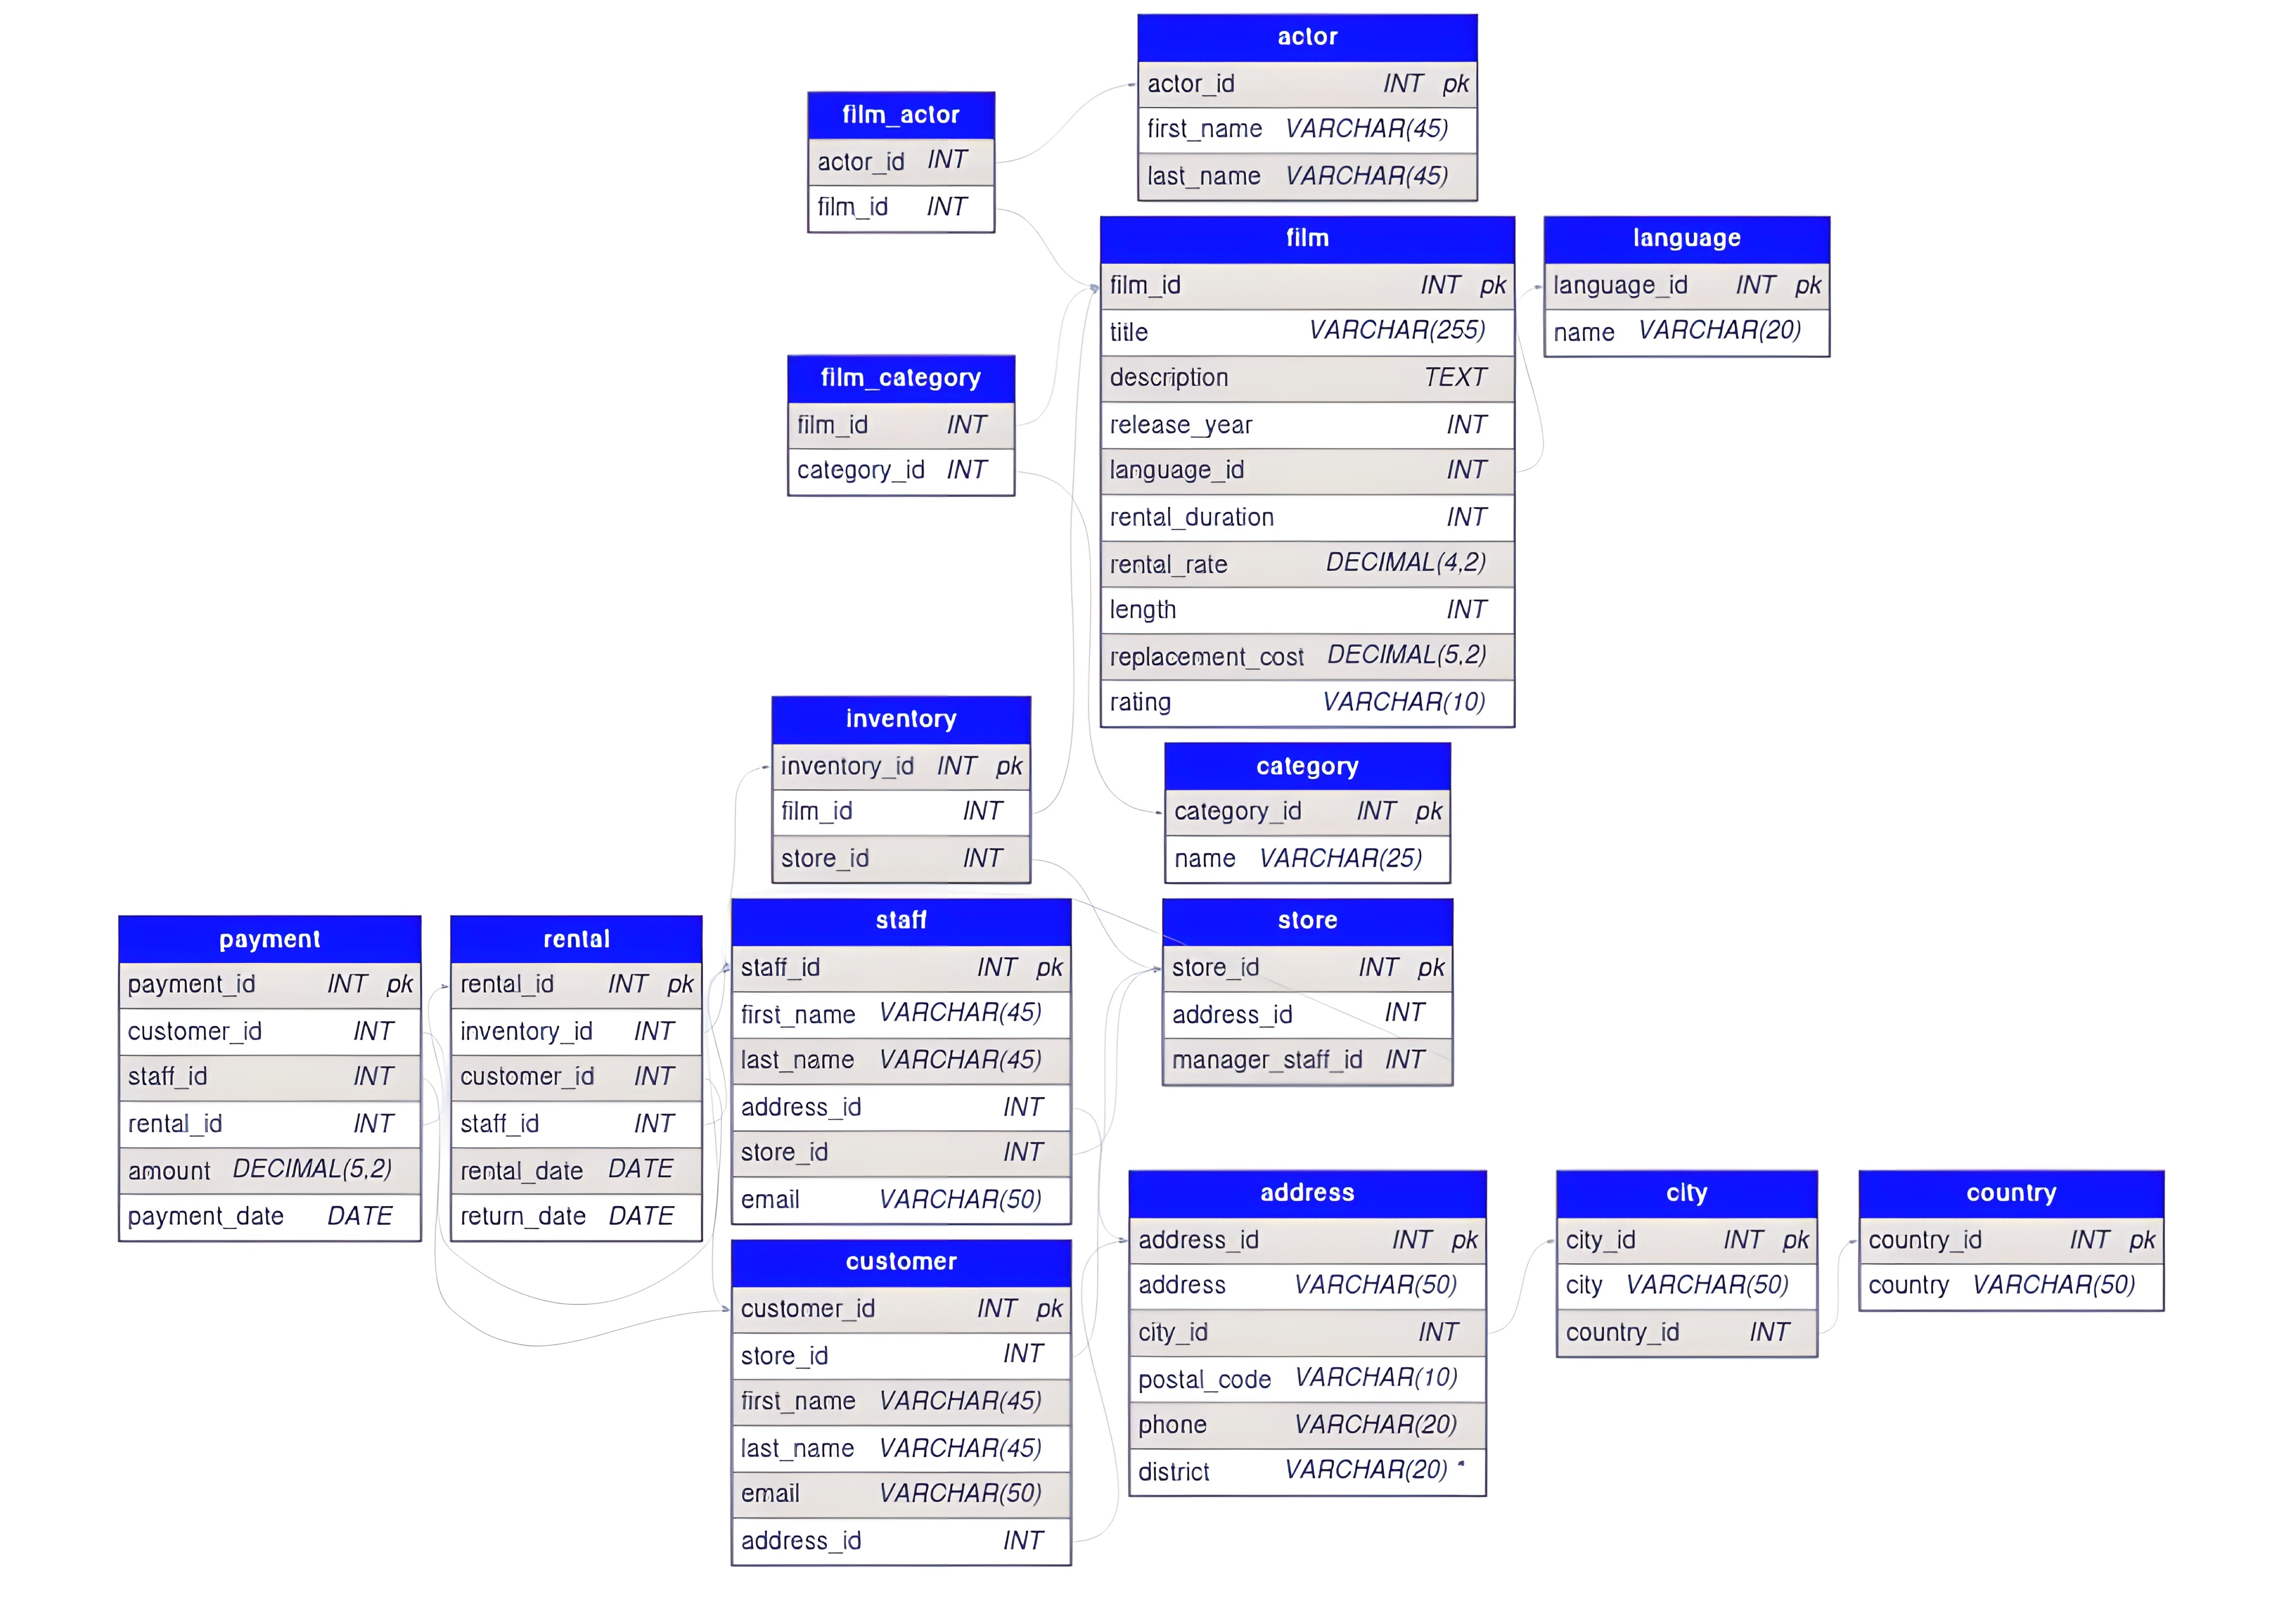
\includegraphics[width=22.5cm]{lab_08_dvdrental_1.png}
\end{figure}

\begin{enumerate}

    \item Find the rentals that did not cross a calendar boundary between rent and return.

    \ifshowsolutions
    \begin{lstlisting}[language=SQL]
    SELECT rental_id, rental_date, return_date
    FROM rental
    WHERE EXTRACT(MONTH FROM rental_date) =
          EXTRACT(MONTH FROM return_date);
    \end{lstlisting}
    \fi

\item List all customers whose email contains their first name.

\ifshowsolutions
\textbf{Solution:}
\begin{lstlisting}[language=SQL]
SELECT first_name, last_name, email
FROM customer
WHERE POSITION(LOWER(first_name) IN LOWER(email)) > 0;
\end{lstlisting}
\fi

    \item Show the total number of rentals that have been returned and the total number that have not been returned yet, as separate rows.

    \ifshowsolutions
    \begin{lstlisting}[language=SQL]
    SELECT 'Returned' AS status, COUNT(*) AS total
    FROM rental
    WHERE return_date IS NOT NULL

    UNION ALL
    
    SELECT 'Not Returned' AS status, COUNT(*) AS total
    FROM rental
    WHERE return_date IS NULL;
    \end{lstlisting}
    \fi

    \item Display the title of films that end with a consonant.

    \ifshowsolutions
    \begin{lstlisting}[language=SQL]
    SELECT title
    FROM film
    WHERE LOWER(title) NOT LIKE '%a'
      AND LOWER(title) NOT LIKE '%e'
      AND LOWER(title) NOT LIKE '%i'
      AND LOWER(title) NOT LIKE '%o'
      AND LOWER(title) NOT LIKE '%u';
    \end{lstlisting}
    \fi

    \item Find all customers whose first name starts with the letter \texttt{A}.

    \ifshowsolutions
    \begin{lstlisting}[language=SQL]
    SELECT first_name, last_name
    FROM customer
    WHERE first_name LIKE 'A%';
    \end{lstlisting}
    \fi

    \item Identify the film categories that contain more than 50 films.

    \ifshowsolutions
    \begin{lstlisting}[language=SQL]
    SELECT c.name, COUNT(fc.film_id) AS film_count
    FROM category c
    JOIN film_category fc ON c.category_id = fc.category_id
    GROUP BY c.name
    HAVING COUNT(fc.film_id) > 50;
    \end{lstlisting}
    \fi

    \item Find out which customers have rented films from more than one store.

    \ifshowsolutions
    \begin{lstlisting}[language=SQL]
    SELECT c.customer_id, c.first_name, c.last_name
    FROM customer c
    JOIN rental r ON c.customer_id = r.customer_id
    JOIN inventory i ON r.inventory_id = i.inventory_id
    GROUP BY c.customer_id, c.first_name, c.last_name
    HAVING COUNT(DISTINCT i.store_id) > 1;
    \end{lstlisting}
    \fi

    \item For each year, find the total number of rentals made in that year.

    \ifshowsolutions
    \begin{lstlisting}[language=SQL]
    SELECT EXTRACT(YEAR FROM rental_date) AS year,
           COUNT(*) AS total_rentals
    FROM rental
    GROUP BY year
    ORDER BY year;
    \end{lstlisting}
    \fi

    \item Find customers who have rented films from ten different categories.

    \ifshowsolutions
    \begin{lstlisting}[language=SQL]
    SELECT customer_id, first_name, last_name
    FROM customer
    WHERE customer_id IN (
        SELECT r.customer_id
        FROM rental r
        JOIN inventory i ON r.inventory_id = i.inventory_id
        JOIN film_category fc ON i.film_id = fc.film_id
        GROUP BY r.customer_id
        HAVING COUNT(DISTINCT fc.category_id) = 10
    );
    \end{lstlisting}
    \fi

\item List the customers who have spent more money in total than the average total amount spent by a customer.


\ifshowsolutions
\textbf{Solution:}
\begin{lstlisting}[language=SQL]
SELECT 
    c.first_name, 
    c.last_name, 
    SUM(p.amount) AS total_paid
FROM customer c
JOIN payment p ON c.customer_id = p.customer_id
GROUP BY c.customer_id
HAVING SUM(p.amount) > (
    -- Subquery: Calculate the Average of the Totals
    SELECT AVG(total_per_customer)
    FROM (
        -- Inner Subquery: Calculate Total per Customer first
        SELECT SUM(amount) AS total_per_customer
        FROM payment
        GROUP BY customer_id
    ) AS derived_table
);
\end{lstlisting}
\fi

\end{enumerate}

\end{document}